\subsection{Pruebas de sistema}
Esta prueba tiene como objetivo verificar que se han integrado adecuadamente todos los elementos del sistema y que realizan las operaciones apropiadas funcionando como un todo \citep{sommerville2011software}.
\subsubsection*{M�todo de prueba de caja negra:}
Las pruebas de caja negra se centran en los requisitos funcionales del sistema. Con estas pruebas se intentan encontrar funciones incorrectas o ausentes, errores de interfaz, errores en estructuras de datos o en acceso a base de datos externas y errores de rendimiento. Se centran en qu� hace el software y no en c�mo lo hace \citep{pressman_isw_7ma}.
Seg�n \citep{pressman_isw_7ma} existen varias t�cnicas para realizar este tipo de pruebas,
se seleccion� la t�cnica partici�n equivalente, la cual permite comprobar los valores v�lidos e
inv�lidos de las entradas existentes en la aplicaci�n.
\paragraph*{Partici�n equivalente:} m�todo que divide el campo de entrada de un programa en clases
de datos de los que se pueden derivar casos de prueba. Se dirige a la definici�n de
casos de prueba que descubran clases de errores, reduciendo as� el n�mero total de
casos de prueba que hay que desarrollar.
La figura \ref{fig:tests-system-coverage} a continuaci�n muestra el resultado de la aplicaci�n de esta prueba.

\clearpage
\begin{figure}[htp]
	\centering
	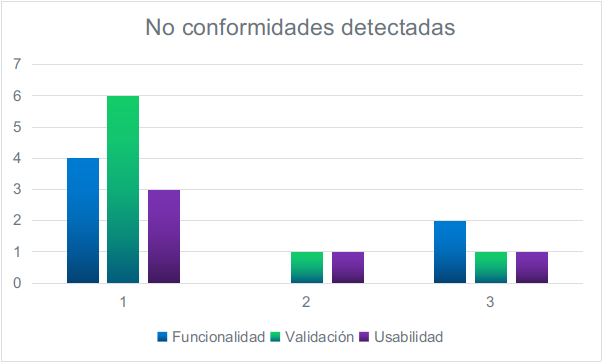
\includegraphics[width=0.8\textwidth]{images/test/no-conf.png}
	\caption{No conformidades detectadas}
	\label{fig:tests-system-coverage}
\end{figure}